\section{Introduction}
\label{sec:intro}

\subsection{A Great Theorem}
The Gauss-Bonnet theorem relates the curvature, a local property, of a surface to the 
to the Euler characteristic, a global property. In symbols 

\begin{equation}\label{eqn:g-b-noboundary}
		\int_MK dA =2\pi \chi(M)
\end{equation}
where $M$ is a smooth surface in $\RR^3$ without bounary, $K$ is Gaussian curvature
and $\chi(M)$ is the Euler characteristic of $M$.
The theorem is a bridge between many ideas that may
seem separate at first, see \figref{bridge}. 




\begin{figure}[htb]
\centering
\includegraphics[width=.3\textwidth]{curvature/bridge}
\caption{The Gauss-Bonnet theorem is a star.}
\label{fig:bridge}
\end{figure}

In the book \emph{Using the Borsuk-Ulam Theorem}
\cite{jm08},
Matou\v{s}ek states that a theorem is a great theorem if there are
\begin{enumerate}[(1)]
\item several different equivalent versions,
\item many different proofs,
\item a host of extensions and generalizations, and
\item numerous interesting applications.
\end{enumerate}

By this criteria, the Gauss-Bonnet theorem is a great theorem.
For (1), six\todo{verify} different versions of the theorem are discussed
in \cite{wu_historical_2008}. 
In addition to the version for smooth surfaces given in \eqnref{g-b-noboundary},
we highlight
 several discrete versions for triangulated surfaces. 
  




 
 
As for (2), several fundamentally different proofs exist.  
One common approach is to first prove the theorem for simply connected domains
with boundary, then triangulate a surface and add up the contribution from each triangle.
However, this proof seems to lack a geometric intuition that other proofs provide. \cite{wu_historical_2008},
A second commonly seen proof is to use Stokes theorem  \cite{doc76,pressley_elementary_2010}.
Many other proofs exist \cite{guillemin_differential_2010,levi-bicycle,grinfeld_introduction_2013}.


For (3), the theorem has been generalized in many ways.
The two notable examples are the Chern-Gauss-Bonnet theorem\cite{chern_simple_1944} and
the Atiyah–Singer index theorem is an example  \cite{atiyah_index_1963}.
A generalization to higher dimensions \cite{guillemin_differential_2010}.


As for (4), applications, 
seven are given in \cite{doc76}.
For applications to physics see \cite{tirado-physics-apps,gibbons_applications_2008}.
This work provides many examples related to the algorithms and combinatorics. 
I hope that the number of applications continues to grow,
please share any that you feel
ought to be included\footnote{\text{bradleymccoy@montana.edu}}.


\subsection{Simple Polygons}
\label{sec:warm-up}

To get a sense of the types of problems we will encounter,
we begin by deriving a formula for the area
of a simple polygon on the sphere in terms of the 
interior angles.
\begin{theorem}\label{thm:triangle}
In the plane, the sum of the interior angles of a triangle is $\pi$.
\end{theorem}
\begin{proof}
Draw a line parallel to one edge through the opposite vertex.
By alternating interior angles in the plane, the sum of the angles
in the triangle equal  a straight line.
See \figref{angles} for an illustration. 



\begin{figure}[htb]
\centering
\includegraphics[width=.3\textwidth]{background/interior-angles-triangle}
\caption{A proof that, in the plane, the sum of the angles of a triangle is $\pi$.}
\label{fig:angles}
\end{figure}

\end{proof}



Consider any simple polygon in the plane $P$ with $n$ vertices. 
Then $P$ can be triangulated with $n-2$ triangles \cite{orourke_computational_1994}.
Thus, when we traverse $P$ we go around $n-2$ triangles each contributing
$\pi$.
We have
\begin{corollary}\label{cor:angles}
In the plane, any simple polygon $P$ with $n$ vertices,
the sum of the interior angles of $P$ is $(n-2)\pi$.

\end{corollary}

Now consider a triangle on the two dimensional sphere as in \figref{sphere-triangle}.

\begin{figure}[htb]
\centering
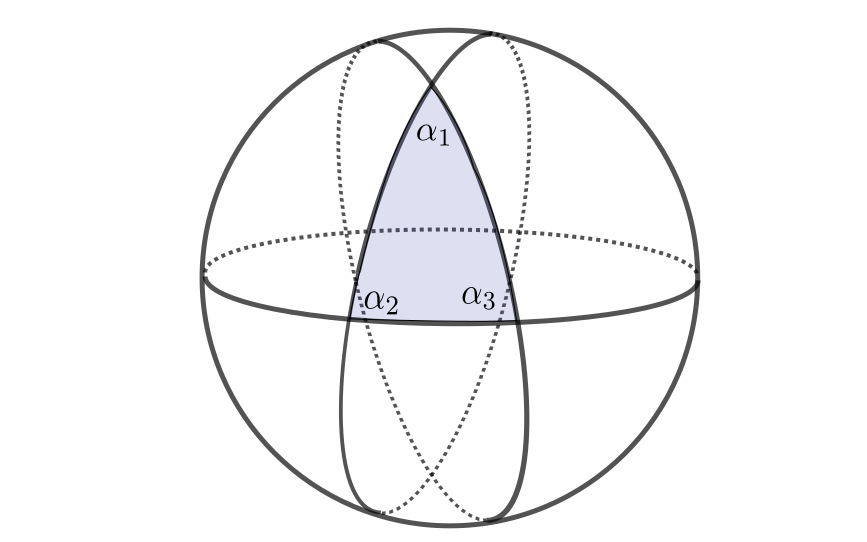
\includegraphics[width=.5\textwidth]{background/sphere-triangle}
\caption{A triangle on the sphere.}
\label{fig:sphere-triangle}
\end{figure}


\begin{figure}[htb]
\centering
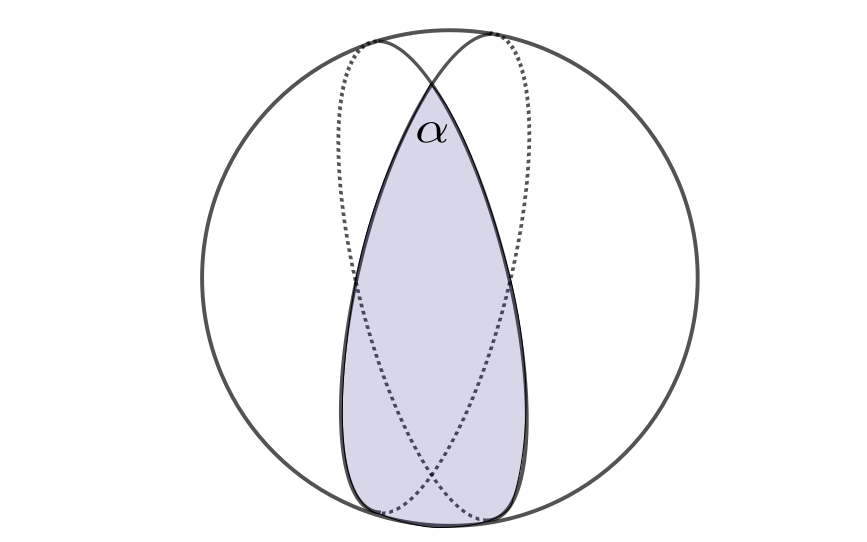
\includegraphics[width=.4\textwidth]{background/lune}
\caption{A lune with angle $\alpha$.}
\label{fig:lune}
\end{figure}

\subsection{Pick's Theorem}
\label{sec:pick}

\cite{og-pick}
\cite{blatter_another_1997}
\cite{tabachnikov_proofs_2014}


